\documentclass[11pt,a4paper]{article}

\usepackage[margin=22mm,headheight=14pt]{geometry}

\usepackage{longtable,booktabs,array,hyperref,xcolor,tikz,fancyhdr}

\usepackage{fontspec,xeCJK}

\setmainfont[Ligatures=TeXOff]{Times New Roman}

\setsansfont[Ligatures=TeXOff]{Times New Roman}

\setmonofont[Ligatures=TeXOff,WordSpace={1,1,1}]{Times New Roman}

\setCJKmainfont{Noto Serif CJK SC}

\setCJKsansfont{Noto Serif CJK SC}

\setCJKmonofont{Noto Serif CJK SC}

\XeTeXgenerateactualtext=1

\definecolor{vulcan}{HTML}{BB3E23}

\pgfdeclarelayer{connections}\pgfdeclarelayer{edge labels}\pgfsetlayers{connections,main,edge labels}

\hypersetup{hidelinks}

\newcolumntype{L}[1]{>{\raggedright\arraybackslash}p{#1}}

\setlength{\emergencystretch}{5em}\tolerance=2000\hbadness=10000

\setlength{\parindent}{0pt}\setlength{\parskip}{5pt}

\pagestyle{fancy}\fancyhf{}\fancyhead[L]{\small\sffamily VULCAN}

\fancyhead[R]{\small Product design and verification}\fancyfoot[C]{\thepage}

\begin{document}

{\sffamily\huge\raggedright\textbf{Anvil-Q1 Phase 2: Official AWQ Checkpoint-Slice Integration and RTL Evaluation}\par}

{\large Technical Design and Verification Report}\par

16 October 2026 (\allowbreak{}UTC+\allowbreak{}8)\allowbreak{}\par\textcolor{vulcan}{\rule{\textwidth}{0.5pt}}

\begin{abstract}

Anvil-Q1 is a modular,\allowbreak{} serialized SystemVerilog accelerator for Qwen2.5 AWQ transformer operations. Phase 2 integrates authentic binary16 and packed I32 checkpoint data through the existing external-memory interface,\allowbreak{} preserving the eight-lane GEMV datapath,\allowbreak{} reused decoder engine and Q16.16 numerical contract.


The bounded official-checkpoint evaluation completed all 14 selected 64x64 projection submatrices from layers 0 and 23,\allowbreak{} covering 57,\allowbreak{}344 products and 896 output writes with zero integer-oracle mismatches. Four-token,\allowbreak{} two-layer top-level execution also matched 6,\allowbreak{}144 scratch/\allowbreak{}cache writes and 256 logits bit-for-bit. Against the independent FP32 baseline,\allowbreak{} aggregate logit cosine similarity was 0.999999299592,\allowbreak{} MAE 0.000706030267 and RMSE 0.000841981995; every token matched the software top-1 and top-5 set. These results establish authentic official-slice execution,\allowbreak{} not full-checkpoint inference [\allowbreak{}E015,\allowbreak{} E024]\allowbreak{}.


\end{abstract}

\section{Architecture and design rationale}

The core processes one token at a time,\allowbreak{} serializing external model,\allowbreak{} scratch and cache accesses through one outstanding memory transaction. A single decoder engine is reused across configured layers; intermediate vectors and context remain external rather than occupying model-sized internal arrays. Each concrete GEMV computes eight output channels concurrently through eight connected dequantizers and wide arithmetic. The decoder and SwiGLU block have separate GEMV instances,\allowbreak{} selected sequentially by control. This architecture prioritizes bounded internal storage and explicit arithmetic over throughput. Packed request selection and operand isolation preserve protocol behavior without establishing a measured power or speed benefit [\allowbreak{}E003,\allowbreak{} E004,\allowbreak{} E011,\allowbreak{} E012,\allowbreak{} E013]\allowbreak{}.

\begin{center}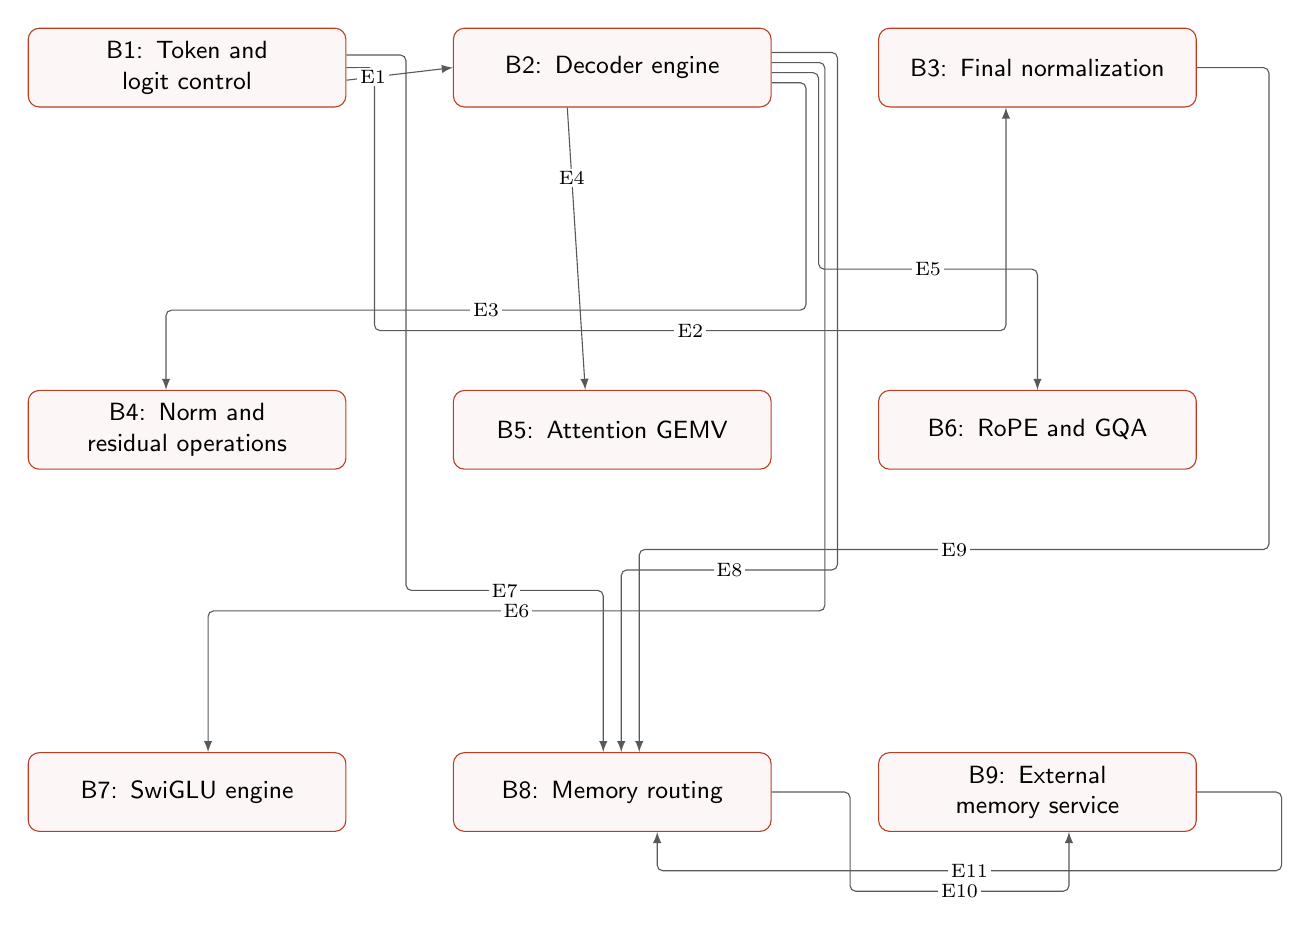
\begin{tikzpicture}[every node/.style={font=\small\sffamily},>=latex]

\node[draw=vulcan,rounded corners,fill=vulcan!4,text width=3.8cm,minimum height=1cm,align=center] (b0) at (0.0,0.0) {B1: Token and logit control};

\node[draw=vulcan,rounded corners,fill=vulcan!4,text width=3.8cm,minimum height=1cm,align=center] (b1) at (5.4,0.0) {B2: Decoder engine};

\node[draw=vulcan,rounded corners,fill=vulcan!4,text width=3.8cm,minimum height=1cm,align=center] (b2) at (10.8,0.0) {B3: Final normalization};

\node[draw=vulcan,rounded corners,fill=vulcan!4,text width=3.8cm,minimum height=1cm,align=center] (b3) at (0.0,-4.6) {B4: Norm and residual operations};

\node[draw=vulcan,rounded corners,fill=vulcan!4,text width=3.8cm,minimum height=1cm,align=center] (b4) at (5.4,-4.6) {B5: Attention GEMV};

\node[draw=vulcan,rounded corners,fill=vulcan!4,text width=3.8cm,minimum height=1cm,align=center] (b5) at (10.8,-4.6) {B6: RoPE and GQA};

\node[draw=vulcan,rounded corners,fill=vulcan!4,text width=3.8cm,minimum height=1cm,align=center] (b6) at (0.0,-9.2) {B7: SwiGLU engine};

\node[draw=vulcan,rounded corners,fill=vulcan!4,text width=3.8cm,minimum height=1cm,align=center] (b7) at (5.4,-9.2) {B8: Memory routing};

\node[draw=vulcan,rounded corners,fill=vulcan!4,text width=3.8cm,minimum height=1cm,align=center] (b8) at (10.8,-9.2) {B9: External memory service};

\begin{pgfonlayer}{connections}

\draw[->,black!65] ([yshift=-0.160cm]b0.east) -- coordinate[pos=0.25] (e0) ([yshift=0.000cm]b1.west);

\draw[->,black!65,rounded corners=2pt] ([yshift=0.000cm]b0.east) -- (2.380,0.000) -- (2.380,-3.340) -- coordinate[midway] (e1) (10.400,-3.340) -- ([xshift=-0.400cm]b2.south);

\draw[->,black!65,rounded corners=2pt] ([yshift=-0.192cm]b1.east) -- (7.860,-0.192) -- (7.860,-3.080) -- coordinate[midway] (e2) (-0.267,-3.080) -- ([xshift=-0.267cm]b3.north);

\draw[->,black!65] ([xshift=-0.571cm]b1.south) -- coordinate[pos=0.25] (e3) ([xshift=-0.343cm]b4.north);

\draw[->,black!65,rounded corners=2pt] ([yshift=-0.064cm]b1.east) -- (8.020,-0.064) -- (8.020,-2.560) -- coordinate[midway] (e4) (10.800,-2.560) -- ([xshift=0.000cm]b5.north);

\draw[->,black!65,rounded corners=2pt] ([yshift=0.064cm]b1.east) -- (8.100,0.064) -- (8.100,-6.900) -- coordinate[midway] (e5) (0.267,-6.900) -- ([xshift=0.267cm]b6.north);

\draw[->,black!65,rounded corners=2pt] ([yshift=0.160cm]b0.east) -- (2.780,0.160) -- (2.780,-6.640) -- coordinate[midway] (e6) (5.286,-6.640) -- ([xshift=-0.114cm]b7.north);

\draw[->,black!65,rounded corners=2pt] ([yshift=0.192cm]b1.east) -- (8.260,0.192) -- (8.260,-6.380) -- coordinate[midway] (e7) (5.514,-6.380) -- ([xshift=0.114cm]b7.north);

\draw[->,black!65,rounded corners=2pt] ([yshift=0.000cm]b2.east) -- (13.740,0.000) -- (13.740,-6.120) -- coordinate[midway] (e8) (5.743,-6.120) -- ([xshift=0.343cm]b7.north);

\draw[->,black!65,rounded corners=2pt] ([yshift=0.000cm]b7.east) -- (8.420,-9.200) -- (8.420,-10.460) -- coordinate[midway] (e9) (11.200,-10.460) -- ([xshift=0.400cm]b8.south);

\draw[->,black!65,rounded corners=2pt] ([yshift=0.000cm]b8.east) -- (13.900,-9.200) -- (13.900,-10.200) -- coordinate[midway] (e10) (5.971,-10.200) -- ([xshift=0.571cm]b7.south);

\end{pgfonlayer}

\begin{pgfonlayer}{edge labels}

\node[fill=white,inner sep=1pt,font=\scriptsize] at (e0) {E1};

\node[fill=white,inner sep=1pt,font=\scriptsize] at (e1) {E2};

\node[fill=white,inner sep=1pt,font=\scriptsize] at (e2) {E3};

\node[fill=white,inner sep=1pt,font=\scriptsize] at (e3) {E4};

\node[fill=white,inner sep=1pt,font=\scriptsize] at (e4) {E5};

\node[fill=white,inner sep=1pt,font=\scriptsize] at (e5) {E6};

\node[fill=white,inner sep=1pt,font=\scriptsize] at (e6) {E7};

\node[fill=white,inner sep=1pt,font=\scriptsize] at (e7) {E8};

\node[fill=white,inner sep=1pt,font=\scriptsize] at (e8) {E9};

\node[fill=white,inner sep=1pt,font=\scriptsize] at (e9) {E10};

\node[fill=white,inner sep=1pt,font=\scriptsize] at (e10) {E11};

\end{pgfonlayer}

\end{tikzpicture}\end{center}

{\small Functional block map, not a gate-level netlist. Edge identifiers match the directed relationships below. Crossings do not denote junctions; separate attachment points preserve arrow directions.}

{\small\begin{longtable}{@{}L{0.24\textwidth}L{0.7\textwidth}@{}}\toprule

\textbf{Block} & \textbf{Responsi\allowbreak{}bility}\\\midrule\endhead

B1: Token and logit control & anvil\_\allowbreak{}q1\_\allowbreak{}top accepts tokens,\allowbreak{} validate\allowbreak{}s sequence position\allowbreak{}s,\allowbreak{} loads embeddin\allowbreak{}gs,\allowbreak{} schedule\allowbreak{}s layers and streams tied-projecti\allowbreak{}on logits.\\[3pt]

B2: Decoder engine & anvil\_\allowbreak{}q1\_\allowbreak{}decoder\_\allowbreak{}layer schedule\allowbreak{}s normaliz\allowbreak{}ation,\allowbreak{} attentio\allowbreak{}n projecti\allowbreak{}ons,\allowbreak{} RoPE,\allowbreak{} GQA,\allowbreak{} residual addition\allowbreak{}s and SwiGLU.\\[3pt]

B3: Final normaliz\allowbreak{}ation & The top-level RMSNorm instance normaliz\allowbreak{}es the final residual before vocabula\allowbreak{}ry projecti\allowbreak{}on.\\[3pt]

B4: Norm and residual operatio\allowbreak{}ns & Decoder-local RMSNorm and elementw\allowbreak{}ise hardware operate on external scratch vectors with defined rounding and saturati\allowbreak{}on.\\[3pt]

B5: Attentio\allowbreak{}n GEMV & The decoder GEMV executes Q,\allowbreak{} K,\allowbreak{} V and O projecti\allowbreak{}ons in eight-output tiles,\allowbreak{} includin\allowbreak{}g QKV biases.\\[3pt]

B6: RoPE and GQA & Split-half rotation and causal grouped-query attentio\allowbreak{}n update external KV storage and produce attentio\allowbreak{}n context.\\[3pt]

B7: SwiGLU engine & anvil\_\allowbreak{}q1\_\allowbreak{}swiglu\_\allowbreak{}mlp contains a separate eight-lane GEMV for gate,\allowbreak{} up and down projecti\allowbreak{}ons,\allowbreak{} plus SiLU and elementw\allowbreak{}ise multipli\allowbreak{}cation.\\[3pt]

B8: Memory routing & Hierarch\allowbreak{}ical muxes and transact\allowbreak{}ion controll\allowbreak{}ers select the active client and isolate inactive response\allowbreak{}s.\\[3pt]

B9: External memory service & Supplies immutabl\allowbreak{}e checkpoi\allowbreak{}nt words,\allowbreak{} mutable scratch/\allowbreak{}KV storage and independ\allowbreak{}ently generate\allowbreak{}d RoPE coeffici\allowbreak{}ents,\allowbreak{} never computed layer outputs.\\[3pt]

\bottomrule\end{longtable}}

{\small\begin{longtable}{@{}L{0.24\textwidth}L{0.7\textwidth}@{}}\toprule

\textbf{Directed relation\allowbreak{}ship} & \textbf{Meaning}\\\midrule\endhead

E1: B1 to B2 & Layer command and completi\allowbreak{}on\\[3pt]

E2: B1 to B3 & Final-normaliz\allowbreak{}ation command\\[3pt]

E3: B2 to B4 & Norm and residual scheduli\allowbreak{}ng\\[3pt]

E4: B2 to B5 & Projecti\allowbreak{}on commands\\[3pt]

E5: B2 to B6 & Rotation and attentio\allowbreak{}n commands\\[3pt]

E6: B2 to B7 & MLP command and completi\allowbreak{}on\\[3pt]

E7: B1 to B8 & Embeddin\allowbreak{}g and tied-logit requests\\[3pt]

E8: B2 to B8 & Selected decoder-subtree requests\\[3pt]

E9: B3 to B8 & Final-norm requests\\[3pt]

E10: B8 to B9 & Serializ\allowbreak{}ed memory requests\\[3pt]

E11: B9 to B8 & Read response\allowbreak{}s and write acknowle\allowbreak{}dgements\\[3pt]

\bottomrule\end{longtable}}

\section{Interfaces and configuration}

{\small\begin{longtable}{@{}L{0.2\textwidth}L{0.12\textwidth}L{0.1\textwidth}L{0.48\textwidth}@{}}\toprule

\textbf{Signal /\allowbreak{} group} & \textbf{Directio\allowbreak{}n} & \textbf{Width} & \textbf{Contract}\\\midrule\endhead

clk,\allowbreak{} rst\_\allowbreak{}n & Input & 1 bit each & Rising-edge clock and synchron\allowbreak{}ous active-low reset. Asserted reset combinat\allowbreak{}ionally gates outward handshak\allowbreak{}es,\allowbreak{} status and payloads to zero; a rising edge clears state. The resetles\allowbreak{}s combinat\allowbreak{}ional dequanti\allowbreak{}zer is exempt.\\[3pt]

token\_\allowbreak{}valid,\allowbreak{} token\_\allowbreak{}ready,\allowbreak{} token\_\allowbreak{}id,\allowbreak{} token\_\allowbreak{}pos,\allowbreak{} new\_\allowbreak{}sequence & Input except token\_\allowbreak{}ready output & 1,\allowbreak{} 1,\allowbreak{} 32,\allowbreak{} 32,\allowbreak{} 1 bits & Transfer\allowbreak{}s sample pre-edge valid \&\& ready. IDs and position\allowbreak{}s must be in range; continua\allowbreak{}tion must use the next committe\allowbreak{}d position. new\_\allowbreak{}sequence is sampled only on acceptan\allowbreak{}ce and requires position zero.\\[3pt]

logit\_\allowbreak{}valid,\allowbreak{} logit\_\allowbreak{}ready,\allowbreak{} logit\_\allowbreak{}index,\allowbreak{} logit\_\allowbreak{}data & Output except logit\_\allowbreak{}ready input & 1,\allowbreak{} 1,\allowbreak{} 32,\allowbreak{} signed 32 bits & Ordered vocabula\allowbreak{}ry-index stream carrying signed Q16.16 logits. Valid,\allowbreak{} index and data remain stable under backpres\allowbreak{}sure. Every configur\allowbreak{}ed logit must transfer,\allowbreak{} includin\allowbreak{}g a singleto\allowbreak{}n first/\allowbreak{}last logit.\\[3pt]

done,\allowbreak{} error & Output & 1 bit each & One-cycle completi\allowbreak{}on with error qualifie\allowbreak{}d by done. Successf\allowbreak{}ul final-logit transfer commits sequence position. Readines\allowbreak{}s remains low during completi\allowbreak{}on.\\[3pt]

mem\_\allowbreak{}req\_\allowbreak{}valid,\allowbreak{} mem\_\allowbreak{}req\_\allowbreak{}ready,\allowbreak{} mem\_\allowbreak{}req\_\allowbreak{}write & Output except mem\_\allowbreak{}req\_\allowbreak{}ready input & 1 bit each & One outstand\allowbreak{}ing transact\allowbreak{}ion; acceptan\allowbreak{}ce samples valid \&\& ready. All request fields remain frozen during stalls. Writes require acknowle\allowbreak{}dgements.\\[3pt]

mem\_\allowbreak{}req\_\allowbreak{}kind,\allowbreak{} mem\_\allowbreak{}req\_\allowbreak{}layer,\allowbreak{} mem\_\allowbreak{}req\_\allowbreak{}proj,\allowbreak{} mem\_\allowbreak{}req\_\allowbreak{}row,\allowbreak{} mem\_\allowbreak{}req\_\allowbreak{}col,\allowbreak{} mem\_\allowbreak{}req\_\allowbreak{}wdata & Output & 4,\allowbreak{} 32,\allowbreak{} 3,\allowbreak{} 32,\allowbreak{} 32,\allowbreak{} 32 bits & Kinds 0..11 identify embeddin\allowbreak{}g,\allowbreak{} qweight,\allowbreak{} qzeros,\allowbreak{} scales,\allowbreak{} QKV bias,\allowbreak{} input norm,\allowbreak{} post norm,\allowbreak{} final norm,\allowbreak{} scratch,\allowbreak{} K cache,\allowbreak{} V cache and RoPE. Projecti\allowbreak{}ons 0..6 identify Q/\allowbreak{}K/\allowbreak{}V/\allowbreak{}O/\allowbreak{}gate/\allowbreak{}up/\allowbreak{}down. Only kinds 8..10 are writable. Unused fields and read write-data are zero.\\[3pt]

mem\_\allowbreak{}rsp\_\allowbreak{}valid,\allowbreak{} mem\_\allowbreak{}rsp\_\allowbreak{}ready,\allowbreak{} mem\_\allowbreak{}rsp\_\allowbreak{}rdata,\allowbreak{} mem\_\allowbreak{}rsp\_\allowbreak{}error & Input except mem\_\allowbreak{}rsp\_\allowbreak{}ready output & 1,\allowbreak{} 1,\allowbreak{} 32,\allowbreak{} 1 bits & Exactly one strictly later response follows each accepted request. Request and response transfer\allowbreak{}s never coincide. Model F16 values occupy the low halfword; packed words and scratch/\allowbreak{}cache values use all 32 bits.\\[3pt]

\bottomrule\end{longtable}}

{\small\begin{longtable}{@{}L{0.23\textwidth}L{0.12\textwidth}L{0.57\textwidth}@{}}\toprule

\textbf{Paramete\allowbreak{}r} & \textbf{Default} & \textbf{Meaning /\allowbreak{} supporte\allowbreak{}d values}\\\midrule\endhead

NUM\_\allowbreak{}LAYERS & 24 & Positive,\allowbreak{} with checked address-product bounds; decoder hardware is reused.\\[3pt]

HIDDEN\_\allowbreak{}SIZE & 896 & Positive; equals NUM\_\allowbreak{}Q\_\allowbreak{}HEADS*\allowbreak{}HEAD\_\allowbreak{}DIM; divisibl\allowbreak{}e by eight and GROUP\_\allowbreak{}SIZE.\\[3pt]

INTERMED\allowbreak{}IATE\_\allowbreak{}SIZE & 4864 & Positive; divisibl\allowbreak{}e by eight and GROUP\_\allowbreak{}SIZE.\\[3pt]

NUM\_\allowbreak{}Q\_\allowbreak{}HEADS & 14 & Positive integer multiple of NUM\_\allowbreak{}KV\_\allowbreak{}HEADS.\\[3pt]

NUM\_\allowbreak{}KV\_\allowbreak{}HEADS & 2 & Positive; NUM\_\allowbreak{}KV\_\allowbreak{}HEADS*\allowbreak{}HEAD\_\allowbreak{}DIM is eight-aligned.\\[3pt]

HEAD\_\allowbreak{}DIM & 64 & Positive and even for split-half RoPE.\\[3pt]

GROUP\_\allowbreak{}SIZE & 128 & Positive divisor of hidden and intermed\allowbreak{}iate dimensio\allowbreak{}ns; need not be a power of two.\\[3pt]

AWQ\_\allowbreak{}BITS & 4 & Only four-bit AWQ GEMM is supporte\allowbreak{}d.\\[3pt]

VOCAB\_\allowbreak{}SIZE & 151936 & Positive; embeddin\allowbreak{}g address product must fit unsigned 32 bits.\\[3pt]

MAX\_\allowbreak{}SEQ\_\allowbreak{}LEN & 32768 & 1..16777215,\allowbreak{} addition\allowbreak{}ally constrai\allowbreak{}ned by cache and coeffici\allowbreak{}ent address products. Paramete\allowbreak{}r products use unsigned 128-bit checks.\\[3pt]

\bottomrule\end{longtable}}

\section{Behavior and corner cases}

\subsection{Transformer execution}

Each configured layer executes input RMSNorm,\allowbreak{} biased QKV projections,\allowbreak{} split-half RoPE with theta=\allowbreak{}1000000,\allowbreak{} causal GQA,\allowbreak{} O projection,\allowbreak{} residual addition,\allowbreak{} post-attention RMSNorm,\allowbreak{} SwiGLU and a second residual. Final RMSNorm precedes projection through the same embedding storage. RMSNorm epsilon is 1e-6; query head h maps to KV head floor(\allowbreak{}h/\allowbreak{}(\allowbreak{}QH/\allowbreak{}KVH)\allowbreak{})\allowbreak{}.

\subsection{Official coordinate mapping}

The top fixture uses (\allowbreak{}L,\allowbreak{}H,\allowbreak{}I,\allowbreak{}QH,\allowbreak{}KVH,\allowbreak{}D,\allowbreak{}G,\allowbreak{}V,\allowbreak{}SEQ)\allowbreak{}=\allowbreak{}(\allowbreak{}2,\allowbreak{}56,\allowbreak{}56,\allowbreak{}14,\allowbreak{}2,\allowbreak{}4,\allowbreak{}56,\allowbreak{}64,\allowbreak{}4)\allowbreak{},\allowbreak{} mapping hardware layers 0/\allowbreak{}1 to checkpoint layers 0/\allowbreak{}23. Embedding rows are [\allowbreak{}0,\allowbreak{}64)\allowbreak{},\allowbreak{} components and norm coordinates [\allowbreak{}0,\allowbreak{}56)\allowbreak{}. Projection inputs are [\allowbreak{}0,\allowbreak{}56)\allowbreak{}; Q/\allowbreak{}O/\allowbreak{}MLP outputs are [\allowbreak{}0,\allowbreak{}56)\allowbreak{},\allowbreak{} K/\allowbreak{}V outputs [\allowbreak{}0,\allowbreak{}8)\allowbreak{}. Metadata accesses select original G128 group zero,\allowbreak{} so fixture G56 changes no accessed metadata. The standalone 64x64 sweeps likewise use group zero. No padding or synthetic model values are supplied.

\subsection{AWQ and fixed-point arithmetic}

Packed qweight/\allowbreak{}qzeros use shifts [\allowbreak{}0,\allowbreak{}16,\allowbreak{}4,\allowbreak{}20,\allowbreak{}8,\allowbreak{}24,\allowbreak{}12,\allowbreak{}28]\allowbreak{} and w=\allowbreak{}(\allowbreak{}q-z)\allowbreak{}*\allowbreak{}s without GPTQ +\allowbreak{}1. Ordinary finite F16 values convert to signed Q16.16 with nearest/\allowbreak{}ties-away rounding and saturation; scales retain unsigned-32 conversion range. Exact signed-37 dequantized weights feed signed-69 products and signed-128 GEMV sums,\allowbreak{} including bias before final rounding. Tied logits use signed-96 accumulation. Partial reductions do not saturate.

\subsection{Nonlinear arithmetic}

RMSNorm uses widened square sums,\allowbreak{} integer square root and reciprocal. RoPE coefficients are signed Q2.30. Attention uses max-subtracted softmax and a range-reduced six-term exponential,\allowbreak{} zero below -16. SiLU uses a sign-stable sigmoid formulation. Required nonfinite data,\allowbreak{} invalid scales and zero denominators produce explicit errors rather than sanitized outputs.

\subsection{Independent floating baseline}

The official FP32 path decodes original F16 bytes directly,\allowbreak{} avoiding the earlier floating baseline's fixed-point-converted model inputs. struct-based binary32 rounding follows every elementary arithmetic operation,\allowbreak{} with separate multiply/\allowbreak{}add and increasing-index reductions. Host math transcendental results are rounded to FP32. Floating RoPE coefficients are generated independently of Q2.30 coefficients; binary64 is used for metric postprocessing.

\subsection{Ordering and recovery}

Acceptance enters busy without immediate request transfer or completion. A request precedes its response by at least one edge. GEMV consumes all eight lane products on the edge following the packed-weight response. Invalid tokens preserve committed sequence state. Memory,\allowbreak{} child or nonfinite-data failures invalidate continuation and require a fresh position-zero sequence. Acknowledged writes are not rolled back; integration must discard obsolete responses after reset.

\section{Verification methods and measured results}

\subsection{Authentic raw-checkpoint provenance}

\textbf{Method.} Standard-library safetensors parsing,\allowbreak{} whole-file and per-tensor SHA-256 validation,\allowbreak{} shape/\allowbreak{}offset checks,\allowbreak{} original-manifest reconciliation and raw-hex excerpt comparison.

\textbf{Result.} Validated 54 extracted tensors against the 627-tensor,\allowbreak{} 168-linear-module inventory and cross-checked 552 excerpt values. Checkpoint SHA-256: f274ceb6\allowbreak{}f71ac3a9\allowbreak{}dd0f10ad\allowbreak{}68007da8\allowbreak{}dedfd102\allowbreak{}ac129b12\allowbreak{}411b26f8\allowbreak{}85a67ef0.

{\small Evidence: E015,\allowbreak{} E024}

\subsection{All official projection submatrices}

\textbf{Method.} Public-interface Icarus simulation of seven 64x64 projections in each of checkpoint layers 0 and 23,\allowbreak{} with independent integer and FP32 calculations.

\textbf{Result.} 14 commands completed; 57,\allowbreak{}344 products and 896 output writes covered; zero bit mismatches. Aggregate projection-component cosine=\allowbreak{}0.999999999973,\allowbreak{} MAE=\allowbreak{}0.0000412546506,\allowbreak{} RMSE=\allowbreak{}0.0000633708054 and maximum absolute error=\allowbreak{}0.000299543142. These are projection metrics,\allowbreak{} not vocabulary-logit metrics.

{\small Evidence: E013,\allowbreak{} E015,\allowbreak{} E024}

\subsection{Four-token official-slice top-level execution}

\textbf{Method.} Software Layer (\allowbreak{}Official HuggingFace FP32/\allowbreak{}FP16 AWQ Weights)\allowbreak{} versus Hardware RTL Output (\allowbreak{}Official HuggingFace W4A16 RTL Execution)\allowbreak{},\allowbreak{} with every ordered write and logit compared to the integer oracle. Tokens 0,\allowbreak{}1 are prefill; tokens 59,\allowbreak{}59 are software-argmax-selected decode at positions 2,\allowbreak{}3.

\textbf{Result.} 4/\allowbreak{}4 tokens completed; zero mismatches across 6,\allowbreak{}144 writes and 256 logits. Concatenated-logit cosine=\allowbreak{}0.999999299592,\allowbreak{} MAE=\allowbreak{}0.000706030267,\allowbreak{} RMSE=\allowbreak{}0.000841981995 and maximum absolute error=\allowbreak{}0.001879334450. Top-1 agreement,\allowbreak{} top-5 overlap/\allowbreak{}5 and exact top-5-set agreement were 1.0 for every token,\allowbreak{} with ascending-index tie-breaking. No saturation or numerical violations were recorded.

{\small Evidence: E012,\allowbreak{} E015,\allowbreak{} E024}

\subsection{Cycle and transaction accounting}

\textbf{Method.} Count elapsed rising-edge intervals from token acceptance to final-logit transfer,\allowbreak{} recording completion retirement separately and partitioning accepted memory traffic by token,\allowbreak{} kind,\allowbreak{} access,\allowbreak{} layer and projection.

\textbf{Result.} Token latencies were 62,\allowbreak{}782; 67,\allowbreak{}013; 71,\allowbreak{}255; and 75,\allowbreak{}507 cycles: 276,\allowbreak{}557 active-token cycles total,\allowbreak{} averaging 69,\allowbreak{}139.25 cycles/\allowbreak{}token. Retirement was one cycle later per token. The stalled run accepted 90,\allowbreak{}952 memory transactions,\allowbreak{} with 4,\allowbreak{}143 request-stall cycles and 58 logit-stall cycles. These are observed stalled timings,\allowbreak{} not a no-stall baseline.

{\small Evidence: E015,\allowbreak{} E024}

\subsection{Retained parameter and numerical regressions}

\textbf{Method.} A/\allowbreak{}B/\allowbreak{}C/\allowbreak{}D each ran seeds 17,\allowbreak{}43,\allowbreak{}89. In L,\allowbreak{}H,\allowbreak{}I,\allowbreak{}QH,\allowbreak{}KVH,\allowbreak{}D,\allowbreak{}G,\allowbreak{}V,\allowbreak{}SEQ order: A=\allowbreak{}(\allowbreak{}2,\allowbreak{}16,\allowbreak{}32,\allowbreak{}4,\allowbreak{}2,\allowbreak{}4,\allowbreak{}8,\allowbreak{}17,\allowbreak{}4)\allowbreak{},\allowbreak{} B=\allowbreak{}(\allowbreak{}2,\allowbreak{}112,\allowbreak{}128,\allowbreak{}14,\allowbreak{}2,\allowbreak{}8,\allowbreak{}16,\allowbreak{}19,\allowbreak{}3)\allowbreak{},\allowbreak{} C=\allowbreak{}(\allowbreak{}1,\allowbreak{}24,\allowbreak{}48,\allowbreak{}6,\allowbreak{}2,\allowbreak{}4,\allowbreak{}3,\allowbreak{}11,\allowbreak{}3)\allowbreak{},\allowbreak{} D=\allowbreak{}(\allowbreak{}1,\allowbreak{}8,\allowbreak{}8,\allowbreak{}2,\allowbreak{}2,\allowbreak{}4,\allowbreak{}8,\allowbreak{}1,\allowbreak{}1)\allowbreak{}. Directed arithmetic,\allowbreak{} protocol,\allowbreak{} reset,\allowbreak{} error and cache tests supplemented these 12 runs.

\textbf{Result.} All passed,\allowbreak{} including non-power-of-two grouping and singleton boundaries. Limits remained 2/\allowbreak{}256 for isolated nonsaturating operations,\allowbreak{} 16/\allowbreak{}256 for final-normalized components and 16/\allowbreak{}256+\allowbreak{}0.01*\allowbreak{}abs(\allowbreak{}reference)\allowbreak{} per nonsaturating logit. Exponential maximum absolute error was 0.0000140080433 against 0.00003 over 4,\allowbreak{}199 comparisons; public SiLU covered 8,\allowbreak{}200 comparisons.

{\small Evidence: E016,\allowbreak{} E024}

\subsection{Sensitivity to meaningful defects}

\textbf{Method.} Disposable mutations exercised wrong lanes,\allowbreak{} omitted biases,\allowbreak{} GQA/\allowbreak{}RoPE errors,\allowbreak{} future/\allowbreak{}stale cache,\allowbreak{} skipped layers and narrowed dequantizer/\allowbreak{}product/\allowbreak{}accumulator arithmetic. Separate fixtures tested corrupted or malformed checkpoint inputs and uncovered coordinates.

\textbf{Result.} The sensitivity check passed with intended functional kills and parser/\allowbreak{}coverage rejections. Compilation failure or timeout was not accepted as a hardware mutation kill; authoritative checkpoint files remained unchanged.

{\small Evidence: E015,\allowbreak{} E016,\allowbreak{} E025}

\subsection{Synthesizable connected hardware}

\textbf{Method.} Yosys hierarchy checking,\allowbreak{} process and memory lowering,\allowbreak{} optimization,\allowbreak{} check -assert and JSON inspection for A/\allowbreak{}B/\allowbreak{}C/\allowbreak{}D.

\textbf{Result.} All four configurations passed with zero latches and substantive sequential state. Both concrete GEMVs retained eight connected lanes consuming all 37 dequantized output bits per lane. These findings establish generic structural integrity,\allowbreak{} not technology-mapped area,\allowbreak{} timing or physical performance.

{\small Evidence: E002,\allowbreak{} E004,\allowbreak{} E011,\allowbreak{} E013,\allowbreak{} E016,\allowbreak{} E026}

\subsection{Icarus toolchain portability}

\textbf{Method.} Matched Icarus 12 and 13 drivers,\allowbreak{} compiler components and runtimes; warning-clean default/\allowbreak{}A/\allowbreak{}B/\allowbreak{}C/\allowbreak{}D elaboration and an identical public-pin configuration-D protocol test on each.

\textbf{Result.} Both majors passed ten elaborations in total and matched-runtime protocol tests,\allowbreak{} including four invalid tokens,\allowbreak{} three reset aborts and one injected memory error per runtime. Explicit component matching prevented incompatible installed tool components from being mixed.

{\small Evidence: E016,\allowbreak{} E027}

\section{Integration and use}

Use rtl/\allowbreak{}anvil\_\allowbreak{}q1\_\allowbreak{}top.sv as the integration boundary,\allowbreak{} compiling rtl/\allowbreak{}anvil\_\allowbreak{}q1\_\allowbreak{}00\_\allowbreak{}pkg.sv before the remaining RTL. Exact arithmetic,\allowbreak{} scratch slots and addresses are documented in design/\allowbreak{}SPEC.md; official-coordinate mapping and precision semantics are in design/\allowbreak{}OFFICIAL\_\allowbreak{}WEIGHTS\_\allowbreak{}EVALUATION.md.


Preserve the mounted official\_\allowbreak{}weights directory and model JSONs. Serve packed I32 words unchanged and F16 values as original low-halfword bits. Embedding and tied-logit reads must resolve to the same storage. Unknown coordinates must fail explicitly,\allowbreak{} never return synthetic defaults.


Provide external scratch,\allowbreak{} KV and RoPE services with stable stalled requests and strictly later responses,\allowbreak{} including write acknowledgements. Apply reset across a rising edge and discard obsolete responses. Submit tokens only on token\_\allowbreak{}ready; drain every logit and require done without error.


Recorded entry commands are \texttt{python3 tests/\allowbreak{}verify.py --check behavior --out evidence/\allowbreak{}verification/\allowbreak{}functional},\allowbreak{} \texttt{python3 tests/\allowbreak{}verify.py --check behavior --probe mutations --out evidence/\allowbreak{}verification/\allowbreak{}sensitivity},\allowbreak{} \texttt{python3 tests/\allowbreak{}verify.py --check synthesis --out evidence/\allowbreak{}verification/\allowbreak{}synthesis} and \texttt{python3 tests/\allowbreak{}verify.py --check portability --out evidence/\allowbreak{}verification/\allowbreak{}portability}. Occupied destinations are refused and must not be overwritten.


Dependencies are Python standard library,\allowbreak{} Icarus iverilog/\allowbreak{}vvp and Yosys; portability additionally requires matched Icarus 12/\allowbreak{}13 toolchains. Read evidence/\allowbreak{}verification/\allowbreak{}official\_\allowbreak{}weights\_\allowbreak{}comparison.json or its functional-directory counterpart for the passed bounded comparison,\allowbreak{} exact provenance,\allowbreak{} per-token metrics and transaction ledger. The checks ran in the supplied environment; separate clean-directory reproduction is not established.


\section{Limitations and acceptance boundary}

The mounted slice is the authoritative Phase 2 evaluation scope,\allowbreak{} not a complete model checkpoint. Layers 1..22,\allowbreak{} most packed input rows and embedding rows beyond 63 were not evaluated. The two-layer fixture preserves authentic selected coordinates and 7:1 GQA but changes head dimension and geometry; it does not establish full 24-layer inference or language-generation quality.


The FP32 baseline specifies reduction and rounding order,\allowbreak{} not equivalence to an unspecified GPU AWQ kernel. Reported RTL greedy agreement is one-step agreement at shared software-selected prefixes,\allowbreak{} not a separately executed autonomous rollout.


Default dimensions were elaborated; functional and generic-synthesis coverage used bounded configurations. No formal all-parameter proof,\allowbreak{} physical implementation,\allowbreak{} clock-frequency measurement,\allowbreak{} timing closure,\allowbreak{} power estimate or silicon throughput claim is provided.


Tokenization,\allowbreak{} sampling,\allowbreak{} physical memory transport and system-level recovery remain external responsibilities. The serialized interface assumes reliable response association and obsolete-response disposal after reset. Completed writes and already transferred logits cannot be retracted.


\appendix\section{Source inventory}

Production inventory: 13 Verilog/\allowbreak{}SystemVerilog files; 1223 nonblank,\allowbreak{} non-comment lines. Source size is not a correctness or quality metric.

{\small\begin{longtable}{@{}L{0.61\textwidth}L{0.15\textwidth}L{0.15\textwidth}@{}}\toprule

\textbf{Producti\allowbreak{}on file} & \textbf{Physical lines} & \textbf{Code lines}\\\midrule\endhead

rtl/\allowbreak{}anvil\_\allowbreak{}q1\_\allowbreak{}00\_\allowbreak{}pkg.sv & 106 & 106\\[3pt]

rtl/\allowbreak{}anvil\_\allowbreak{}q1\_\allowbreak{}awq\_\allowbreak{}dequant.sv & 38 & 38\\[3pt]

rtl/\allowbreak{}anvil\_\allowbreak{}q1\_\allowbreak{}bus\_\allowbreak{}mux.sv & 35 & 35\\[3pt]

rtl/\allowbreak{}anvil\_\allowbreak{}q1\_\allowbreak{}decoder\_\allowbreak{}layer.sv & 107 & 107\\[3pt]

rtl/\allowbreak{}anvil\_\allowbreak{}q1\_\allowbreak{}elementw\allowbreak{}ise.sv & 91 & 91\\[3pt]

rtl/\allowbreak{}anvil\_\allowbreak{}q1\_\allowbreak{}gqa\_\allowbreak{}attentio\allowbreak{}n.sv & 151 & 151\\[3pt]

rtl/\allowbreak{}anvil\_\allowbreak{}q1\_\allowbreak{}mem\_\allowbreak{}port.sv & 49 & 49\\[3pt]

rtl/\allowbreak{}anvil\_\allowbreak{}q1\_\allowbreak{}paramete\allowbreak{}rs.sv & 27 & 27\\[3pt]

rtl/\allowbreak{}anvil\_\allowbreak{}q1\_\allowbreak{}rmsnorm.sv & 113 & 113\\[3pt]

rtl/\allowbreak{}anvil\_\allowbreak{}q1\_\allowbreak{}rope.sv & 97 & 97\\[3pt]

rtl/\allowbreak{}anvil\_\allowbreak{}q1\_\allowbreak{}swiglu\_\allowbreak{}mlp.sv & 75 & 75\\[3pt]

rtl/\allowbreak{}anvil\_\allowbreak{}q1\_\allowbreak{}top.sv & 151 & 151\\[3pt]

rtl/\allowbreak{}anvil\_\allowbreak{}q1\_\allowbreak{}w4a16\_\allowbreak{}gemv.sv & 183 & 183\\[3pt]

\bottomrule\end{longtable}}

\section{Verification record index}

{\small\begin{longtable}{@{}L{0.57\textwidth}L{0.16\textwidth}L{0.17\textwidth}@{}}\toprule

\textbf{Recorded check} & \textbf{Outcome} & \textbf{Executio\allowbreak{}n time (\allowbreak{}s)\allowbreak{}}\\\midrule\endhead

behavior & passed & 419.328\\[3pt]

sensitiv\allowbreak{}ity & passed & 15.016\\[3pt]

synthesi\allowbreak{}s & passed & 89.119\\[3pt]

portabil\allowbreak{}ity & passed & 5.315\\[3pt]

\bottomrule\end{longtable}}

Execution times include tool and provider waiting; they are not hardware latency or model utilization.

{\small\begin{longtable}{@{}L{0.12\textwidth}L{0.82\textwidth}@{}}\toprule

\textbf{Referenc\allowbreak{}e} & \textbf{Original project-relative record}\\\midrule\endhead

E002 & rtl/\allowbreak{}anvil\_\allowbreak{}q1\_\allowbreak{}awq\_\allowbreak{}dequant.sv\\[3pt]

E004 & rtl/\allowbreak{}anvil\_\allowbreak{}q1\_\allowbreak{}decoder\_\allowbreak{}layer.sv\\[3pt]

E011 & rtl/\allowbreak{}anvil\_\allowbreak{}q1\_\allowbreak{}swiglu\_\allowbreak{}mlp.sv\\[3pt]

E012 & rtl/\allowbreak{}anvil\_\allowbreak{}q1\_\allowbreak{}top.sv\\[3pt]

E013 & rtl/\allowbreak{}anvil\_\allowbreak{}q1\_\allowbreak{}w4a16\_\allowbreak{}gemv.sv\\[3pt]

E015 & tests/\allowbreak{}official\_\allowbreak{}weights.py\\[3pt]

E016 & tests/\allowbreak{}verify.py\\[3pt]

E024 & .vulcan/\allowbreak{}engineer\allowbreak{}ing/\allowbreak{}run-0001/\allowbreak{}attempt-0004/\allowbreak{}stdout.log\\[3pt]

E025 & .vulcan/\allowbreak{}engineer\allowbreak{}ing/\allowbreak{}run-0001/\allowbreak{}attempt-0005/\allowbreak{}stdout.log\\[3pt]

E026 & .vulcan/\allowbreak{}engineer\allowbreak{}ing/\allowbreak{}run-0001/\allowbreak{}attempt-0006/\allowbreak{}stdout.log\\[3pt]

E027 & .vulcan/\allowbreak{}engineer\allowbreak{}ing/\allowbreak{}run-0001/\allowbreak{}attempt-0007/\allowbreak{}stdout.log\\[3pt]

\bottomrule\end{longtable}}

\section{Document provenance}

Engineering was independently accepted for the recorded source and evidence identity. This is not exhaustive proof, hardware deployment or physical signoff. The companion REPORT.md records the exact report approval and source manifest, and links the English/Chinese journeys containing original failures and interventions. A report number identifies a generation attempt, not a new hardware revision.

No developer attribution was supplied; none has been inferred.

\end{document}
